%*******************************************************************************
%****************************** Second Chapter *********************************
%*******************************************************************************

\chapter{Background and Literature Review}

\ifpdf
    \graphicspath{{Chapter2/Figs/Raster/}{Chapter2/Figs/PDF/}{Chapter2/Figs/}}
\else
    \graphicspath{{Chapter2/Figs/Vector/}{Chapter2/Figs/}}
\fi

In this chapter we introduce the basic concepts and methods involved in our thesis. We start by introducing machine learning and the various machine learning algorithhms. We introduce the idea of clustering and dictionary learning.The sparse coding and dictionary learning formulations are discussed in this section. Later we discuss the relevant previous work relating to our thesis. In the last section we briefly describe some of the latest work which resembles our work and represents the state of art methods.
\section[Machine Learning]{Machine Learning}

Machine learning is the study dealing with the process to learn characteristic information from data. Given some data, $ X $ , a machine learning algorithm learns a function $ f(X) $ which maps the input X to an output variable $y$ . The learnt model than can be used to make predictions on previously unseen data $X'$.A machine learning algorithm learns the parameters of an adpative model from a training set, typically optimizing a function. The learnt model is then used to make predictions on previously unseen new data. Broadly, machine learning methods can be divided into two subfields, supervised learning and unsupervised learning. In a supervised setting the target labels or values are known for the test set and we focus on predicting the target value for previously unseen data.In an unsupervised setting no such target information is present for the training data and the focus is to learn structure and compact descriptions from the data.\\

In a supervised setting , given a set of labelled  data points known as the training data: $$ T = \{(x_1,y_1),...,(x_n,y_n)\} $$, where $x_i \in X$ and $y_i \in X$ ,we find a function f, which maps any point in the domain of X to its corresponding label in Y.
If Y is a set of discrete values then the it is known as a classifcation problem and if Y is in a continous range then it is a problem of regression.\\

In an unsupervised setting, the task is to find group relations between instances of the unlabeled training dataset with a subsequent aim of categorizing or clustering the data. The algorithm finds the previous unknown structure in the data.\\

The data point $x_i$ is typically represented as a vector comprising of feature values and is known as a feature vector. For example, given a dataset $X =\{x_1,x_2,...,x_m\}$ where $x_i$ is an image patch of size $\sqrt{n}$ x $\sqrt{n}$,each patch can be represented as a vector of length $n$ formed by concatenating the gray scale values. The entire dataset then can be represented as a matrix:
\begin{equation*}
X = \begin{pmatrix}
x_{1,1} & x_{1,2} & \cdots & x_{1,n} \\
x_{2,1} & x_{2,2} & \cdots & x_{2,n} \\
\vdots  & \vdots  & \ddots & \vdots  \\
x_{m,1} & x_{m,2} & \cdots & x_{m,n}
\end{pmatrix}
\end{equation*}

Here each row of the matrix dentoes individual data points and ${x_{i,j}}$ is the gray scale intensities of patch $x_i$ at pixel location j.
%\subsection{Supervised Learning}
%Give a training set of labelled data, supervised learning algorithims fit a model to the training set with the aim of predciting the unknown labels for the test instances ( observations). During the training phase, the algorithms learns the unkown parameters for the model.
%
%[Describe the process]
%
%[Example of a learning algorithm]
%
%\subsection{Unsupervised Learning}
%
%In unsupervised learning settings, the task is to find group relations between instances of the unlabeled training dataset with a subsequent aim of categorizing or clustering the data. The algorithm aims to understand the general properties/structure in the dataset.
%
%[Explain the method]

\section{Clustering}
A cluster is collection of data points grouped together on basis of some common properties.The data objects or points within a cluster are similar to each other, whereas the points in different groups are disimilar.\\

The process of partioning the data points into smaller groups (called as clusters) with an aim to minimize the intra cluster variance and maximize the inter cluster variance, is known as clustering. The grouping of data points is based on the similarity or disimilarity of the objects as described by their properties or features.\\

Similarity or disimilarity between two objects can be very subjective and hence various measures are used to describe them quantitatively with distance measure being the most common.The distance measure is used to specify the distance between two objects and can be used to create a distance matrix called as similarity/disimilarity matrix. The most commonly used distance metric is the Eucledian Distance.\\

The eucledian distance D between two points $p =\{x_1, x_2, ... , x_n\}$ and $q =\{y_1, y_2, ... , y_n\}$ can be defined as:
\begin{equation}\label{eq: eucledian dist}
\begin{split}
dist(p,q) =  \sqrt{(x_1 - y_1)^2 + (x_2 - y_2)^2 + ... +(x_n - y_n)^2 } \\
		 =  \sqrt{\sum_{i=1}^{n}(p_i - q_i)^2} \\
		 = \lVert \mathbf{p-q} \rVert
\end{split}
\end{equation}

As the data labels are unknown,cluster analysis is known as an unsupervised method of data partionining.This is in contast to classification where the data can be partitioned on the basis of their class labels. Thus, clustering segments the data based on properties of the objects within the dataset and finds previously unkown grouping within the data.

\subsection{K-Means Clustering}\label{sec:kmeans}
In this section we look into the K-Means clustering algorithm (\citet{macqueen1967some}). We assume that the number of clusters 'K' is given and we use it to initiate our clustering algorirthm. The idea is to partition the dataset into 'k' clusters and assign 'k' centorids , one for each cluster \\

Given a datast D =$[x_1,x_2,...,x_n]$ consisting of n objects ,where each object is a feature vector of length 'm'.The clustering algorithm partitions the dataset into 'K' clusters $C_1,C_2...C_k$ such that $C_i$ $\subset$ D and $Ci \cap Cj = \emptyset$ and with an aim to have a low intra cluster varianace and a high inter cluster varianace.This means that the points within the same cluster musts be highly similar and disimilar to the points belogning to other clusters.\\

The partioning is performed in an iterative manner and follows what is known as Lloyd's algorithm\cite{lloydsalgo}. We inititialze the 'k' centroid by some initialization methods such as k-means++ or random initilization.The cluster quality depends on a goood initialization.We start by assigning each point in the dataset to the nearest neareast centroid and we get 'k' clusters. We then calculate the mean points of the new clusters and assign them as the new centroids. The process then continue till a stopping criterion is reached. The partioning is made with an aim to minimize the objective function which is the withing cluster sum of squared error.

Each of the clusters $C_i$ consists of p points and is represented by its centroid $c_i$.The distance between point p and the cluster centre ci is defined as dist(p,ci). If the data points are in m dimensional , then the distance can be computed as in Eq \ref{eq: eucledian dist}. We can then write our objective function J as :
\begin{equation}
J = \sum\limits_{j=1}^{K} \sum\limits_{i=1}^{p} {\lVert\mathbf{x^{(j)}_i - c_j}  \rVert}^2
\end{equation}

K-means clustering is the simplest unsupervised learning algorithm and can be applied to many different problems. An example of K-Means clustering on a toy dataset with 2 clusters is shown in Figure \ref{fig:kmeansvisz}
\begin{figure}
	\centering
	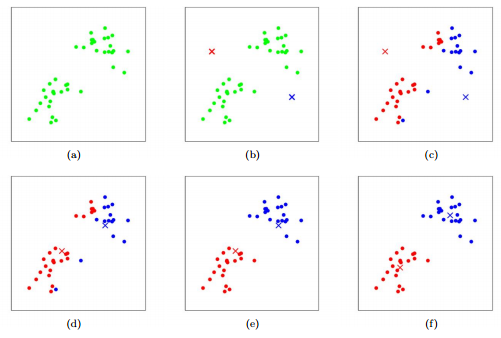
\includegraphics[width=\textwidth]{kmeansViz}
	\caption[K-Means Visualization]{ K-means algorithm. Training examples are shown as dots, and cluster centroids are shown as crosses. (a) Original dataset. (b) Random initial cluster centroids. (c-f) Illustration of running two iterations of k-means. In each iteration, we assign each training example to the closest cluster centroid (shown by "painting" the training examples the same color as the cluster centroid to which is assigned); then we move each cluster centroid to the mean of the points assigned to it. (Images courtesy of Michael Jordan. Retrieved from : http://stanford.edu/~cpiech/cs221/handouts/kmeans.html)}
	\label{fig:kmeansvisz}
\end{figure}

\section{Spare Coding and Dictionary Learning}\label{sec:dlsparse}
The process of learning a finite set of basis elements ,called atoms, from a given training set of signals $X=[x_1,x_2,...,x_n], $ such that each signal in X can be approximately reconstructed by a linear combiantion of atoms is called Dictionary Learning. This finite sets of atoms is called D, is the learnt dictionary. Normally we want to find a sparse decomposition of signals in D i.e, we aim to create a dictionary of sparse elements. This kind of decomposition is different from PCA where the basis elements have to be orthogonal to each other and these dictionaries are in general overcomplete.\\

By overcomplete here we mean that if any element from the dictionary is removed, we can still approximately construct the signal from the atoms. Also the number of atoms in dictionary is of a greater dimension than the data. \citet{lewicki2000learning} describes the process of learning overcomplete set of representations.Some recent work \citep{mairal2009supervised} has shown that sparsity captures high-order correlation in data and it captures higher order statistics in data.\\
 
\citet{huang2006sparse} talks about how to represent a given signal as a sparse decomposition of a dictionary D. In a sparse coding task, our goal is to represent a signal $x \in \mathbb{R}^m$, as a linear comibination of an overcomplete dictionary $D =[d_1,d_2,...,d_k] \in \mathbb{R}^{n x k}$. Here 'k' is the no of atoms $d_k \in \mathbb{R}^n$. To ensure that the dictionary is overcomplete, we have $k > n$. The task is to find a representation in form a sparse code vector $\alpha$ of k x 1, such that:
\begin{equation}\label{eq: sparse coding}
 \alpha = \underset{\alpha '}min {\lVert\alpha \rVert}_0 ,\ \ s.t \ \ x = D \alpha , 
\end{equation}
\\
where $\lVert x \rVert_0$ is l0 norm, which represents the number of non-zero components in x.\\

It has been found that this problem is hard to solve and thus we replace l0-norm with l1-norm, so then as others (\citet{lee2006efficient} , \citet{donoho2006compressed}), the problem is reformulated to find $\alpha$ by mininimizing the objective function J:
\begin{equation}
J(\alpha; \lambda_1) = \underset{\alpha \in \mathbb{R}^k}{min} {\lVert \mathrm{x-D\alpha} \rVert}^2_2 + \lambda_1 \lVert \alpha \rVert
\end{equation}
where the parameter $\lambda_1$ is the regularization parameter which ensures a trade off in sparsity and reconstruction error. It also ensures that the sparse codes are not very large.\\

To further ensure that the dictionary values D, do not become arbitarily large,\citep{mairal2009online} constarin the columns of D to have an l2-norm less than or equal to one. They call the convex set of matrices verifying this constrain as :

For our purpose we use the Online dictionary learning implementation of \citep{mairal2009online}. This is a very efficient methods and works brilliantly for millions of training examples.
Sparse coding is done using the orthogonal matching pursuit (OMP) method  \cite{pati1993orthogonal,tropp2007signal} implemented in the SPAMS libary provided by \citet{mairal2010online}


\section{Literature Review}
In this chapter we aim to present a general overview of vessel segmentation methods.We particularly focus on approaches based on machine learning methods both supervised and unsupervised techniques. There has been a considerable work in the domain of automatic retinal vessel segmentation. \citet{surveyretinal} give a complete review of retinal vessel segmentation methods. We briefly outline some of the methods before we move on to explain the most recent supervised learning based algorithms.\\

The earliest work on retinal segmentations are based on tracking methods to trace the blood vessels\cite{trackingchutatape1998retinal,trackingtolias1998fuzzy}..In these methods the vessel is traced out from some starting seed points according to some relevant criterion. Recently,\citet{vlachos2010multi} proposed a methods based on multi scale line tracking. They approach the problem by tracking the retinal vessel at multi scales and combining the individual image maps at different scales.\citet{farnell2008enhancement} employ multi scale line operators at various orientations to enhance the blood vessels.\\

There has been a recent surge in utilzing supervised machine lerning based methods for vessel segmentation. In such methods, generally, each image pixel is represented as a feture vector computed using local or gloabl information. A classifier is then trained to label every pixel to a vessor or background. Such classifiers rely on the training dataset, which is not available easily.\citet{ricci2007retinal} proposed a supervised classifier using line operators and using support vector classification. They obtain unsupervised pixel classifcation by thresholding the response of basic line detector. Additionaly, they use orthogonal line detectors along with grey level of target pixel to construct feature vector for support vector machines based supervised classification.\citet{staal2004ridge} proposed a ridge based vessel segmentation method used together with a supervised learning technique.\citet{nguyen2011effective} proposed a method utilzing gabor filter responses at multiple scales as features for pixel classification.\cite{vega2013blood,gardner1996automatic} proposed neural network bases approach to vessel segmentation\\

We now look in detail some of the recent state-of-art work on retinal vessel segmentation.

\citet{dollar2013structured} recently proposed a structured learning framework for predicting local edges utilizing random forests.The work exploits the presence of local structure forms like straight lines or T-junctions in image patches to lean an accurate edge detector. They train random forests in structured output spaces. Local image labels are highly interdependent and utilzing the knowledge on such local structures tend to imprtove the the classifiers accuracy. The problem of edge detection is formulated in a way to predict local segmentation maps for input image patches.  The structure labels are mapped to proxy discrete labels, in a way that similar structure labels are assigned to same discrete labels. Using this proxy mapping, existing random forest training approaches are used to learn structured random forests. Finally these forests are used to label each pixel to denote the presence or absence of edges.\\

\citet{rigamonti2012accurate} proposed a method to learn ad hoc features with learned filters.Many hand crafted features have been proposed to solve the problem of extracting linear structures like blood vessels, but are not always effective.In contrast, learned features are better at the task but are computationally expensive. The proposed algorithm complements handcrafted features with learned filters. Linear filters are computed from training images in a convolutional approach. The convolutional filters are constrained to be be dissimilar. Further, feature maps are computed by convolving the learned filters with the images. Several such feature maps our computed both for handcrafted features like(OOF,EF) and for learned filters. These features maps are then used to calculate descriptors at each image location. A random forest classifier is then trained to classify each image pixel as lying on a linear structure or background.\\

\citet{ganin2014n} proposed a very elegant approach to natural edge detection or thin object segmentation. They employ a combination of convolutional neural networks with the neareast neighbor search. The problem is approached in a patch based framework, where the predictions are made patch by patch.